The microscope is a device that performs extremely important tasks to human knowledge, in theoretical or empirical aspects. It is capable of providing magnified views of small objects and structures. Currently, several variations of microscopes are used to investigate much smaller spaces than those visible to the naked eye \cite{wu2008microscope}. Fields such as materials sciences and biology broadly apply microscopy and health professionals use them on large scale for practical procedures, clinical analysis, and research. High throughput microscopy is an important technique for the diagnosis and treatment of genetic diseases. However, to make it acceptable in the clinical environment, it is of great importance to perform high-resolution image acquisition, since low levels of sharpness can directly affect the diagnostic accuracy \cite{qiu2013evaluations}.

The current advances in microscopy technologies and methods show a natural trend of linking novel microscopy improvements and image processing. This bond dates back to the middle of the 20th century, when some techniques for capturing and manipulating images, primarily developed for televisions, were applied to microscopy images \cite{wu2008microscope}. A classic example is noise reduction, which is an important step for cryoelectronic microscopy and also for energy filtering in transmission electron microscopy, before the 3D reconstruction process on Computed Tomography scans. High noise levels hinder the necessary alignment in the reconstruction task \cite{vyas2017multiscale}.

\section{Motivation}

Biological and biomedical analysis procedures using microscopy images also employ image processing algorithms to produce better results. In this scenario, the concept of focus is an element of great relevance. The microscopically analyzed surfaces and structures are \emph{a priori} smooth and homogeneous to the naked eye; when magnified, these images show that those elements are irregular, i.e. they have different depths (when considering an upper view), textures and topologies. It is, therefore, necessary to constantly adjust the focus to obtain a sharp image. \autoref{fig:ctenanthe_blur} illustrates the problem of differences in depth of focus in histological images of a \emph{Ctenanthe oppenheimiana} specimen with the structure of a slope, acquired in the same scene but with different height settings for the objective lenses. The axial location for \autoref{fig:ctenanthe_blur}.(a) was higher than in \autoref{fig:ctenanthe_blur}.(b), and this produced clear differences among the blurred and sharp regions of both images.

\begin{figure}[ht]
    \centering
    \caption{Examples of \textit{Cthenante oppenheimiana} partially blurred images, with the leftmost (a) and rightmost parts (b) as sharp due to topological height differences.}
    \label{fig:ctenanthe_blur}
    \begin{subfigure}[t]{0.45\textwidth}
        \centering
        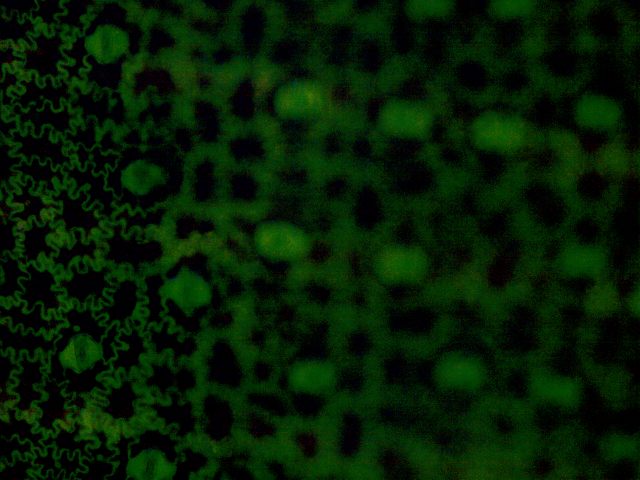
\includegraphics[scale=0.31]{images/cthenante_left.png}
        \caption{}
    \end{subfigure}%
    ~ 
    \begin{subfigure}[t]{0.45\textwidth}
        \centering
        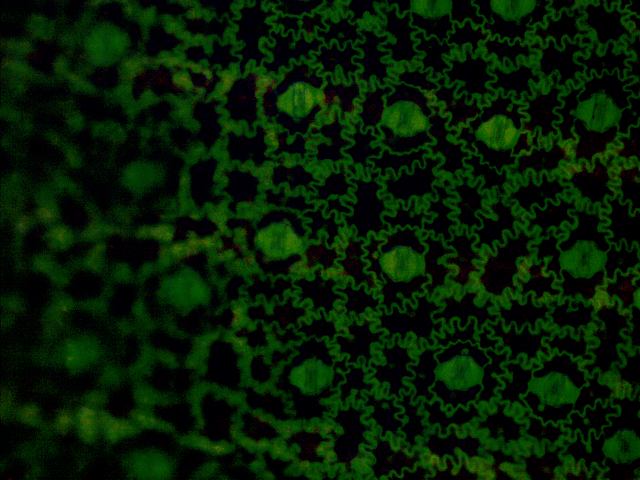
\includegraphics[scale=0.31]{images/cthenante_right.png}
        \caption{}
    \end{subfigure}
    \centering
    \fautor
\end{figure}

Sharpness is a concern when it comes to the analysis of microscopy images in order to obtain conclusions. According to \citeonline{costa2019multi}, blurred regions in sputum smear microscopy images caused by the depth of field limit in the microscope affect the accuracy of bacilli detection. Several proposed methods address the sharpness problem in microscopy images based on image restoration techniques. As stated by \citeonline{ponti2016image}, the most frequently used iterative method in microscopic image restoration is the Richardson-Lucy algorithm. Some examples presented by \citeonline{sun2005autofocusing} consist of four classes: \emph{derivative algorithms}, \emph{statistical algorithms}, \emph{histogram-based algorithms} and \emph{intuitive algorithms}. Among these applications, derivative methods deserve more credit. The Fourier Transform proved itself to be effective for low or moderate noise levels; in highly noisy environments, the resulting images were not satisfactory \cite{richardson1972bayesian}. As a consequence, probabilistic methods based on the Bayes Theorem were developed and provided images with better contrast, higher bandwidth and edge enhancement for confocal fluorescence microscopy samples \cite{ponti2016image}.

The resulting images from such restoration processes are sharper than the observed ones. However, the algorithms produce degradation as output. An alternative to restoration is to use images from the same object, with different foci, in order to obtain an enhanced depth of field image with low degradation levels. This process is known as image fusion, and even though a significant effort was done by researchers towards the development of techniques in this context, most of the image fusion methods are applicable but not directly related and built for bright-field microscopy images. The fusion process also require the selection of images that have ate least some sharp region, and according to \citeonline{koho2016image}, very few publications that address the problems of measuring the quality of images can be found on microscopy applications. There are many image analysis tools, but not many easily accessible and applicable image quality assessment methods.


\section{Aims and Hypothesis}

This work aims to develop a method to perform the fusion of bright-field microscopy images acquired in different focal planes. We propose three stages to achieve this, described as follows:

\begin{itemize}
    \item \emph{Dataset acquisition}: Acquisiton of a bright-field microscopy image dataset of leaf samples to evaluate the performance of the methods;

    \item \emph{No-reference image quality assessment}: Development of a method to quantitatively assess the quality of bright-field microscopy images based on the Fourier transform and descriptive statistics; 
    
    \item \emph{Multi-focus image fusion}: Fusion of the sharp regions of selected images among the dataset by means of a Laplacian of Gaussian-based method and compose the sharp image.
    
\end{itemize}

It is hypothesized that frequency domain information from images may be used to quantify the sharpness of bright-field microscopy images. Simultaneously, we also have the hypothesis that image fusion methods that employ edge detection by means of the Laplacian operator and its derivatives, e.g. the Laplacian of Gaussian, perform well on bright-field microscopy images. 

\section{Contributions}

This work yields the bright-field microscopy z-stack datasets as a first contribution. Those may be used to study, develop and test novel no-reference image quality metrics and multi-focus image fusion techniques by image processing and microscopy researchers, as well as industry professionals. The datasets comprise real world high-resolution microscopy images of biological material (particularly, plant leaves) with different illumination techniques and settings, which turns image quality assessment and image fusion into more challenging tasks.

In addition to the datasets, our proposed quality index and fusion algorithms explore well-known mathematical analysis, image processing, signal processing and statistical techniques. This not only it provides significant applications of those tools, but also stimulates studies among researchers in order to combine new state-of-the-art technologies to strong theoretical concepts in order to develop robust and scalable solutions.

\section*{Structure of the document}

This monograph is organized as follows:

\begin{itemize}
    \item \autoref{chapter:fundamentals-of-optics-and-light-microscopy} provides the bright-field microscopy basics and the z-stacking technique, i.e. the method to acquire images in different focal planes;
    
    \item \autoref{chapter:blur-characterization-and-image-formation} comprises relevant information about the bright-field microscopy image formation process and also describes the defocus blur property;
    
    \item \autoref{chapter:theoretical-background} provides the theoretical basis of this work, i.e. Fourier transform, image enhancement, registration, fusion and quality assessment, as well as the statistical methods employed in the analysis;
    
    \item \autoref{chapter:related-work} presents methods in which this work is based on, by means of a literature review on no-reference image quality assessment and multi-focus image fusion;
    
    \item \autoref{chapter:materials-and-methods} presents the acquisition and usage protocols of the proposed image datasets and the proposed method;
    
    \item \autoref{chapter:results} presents our results with the proposed datasets and exposes a discussion concerning the quantitative and qualitative analysis of them;
    
    \item \autoref{chapter:conclusions} summarizes what has been achieved, suggests some future work on the field and improvements to the methods;
    
    \item
    \autoref{chapter:fundamentals-of-optics} presents fundamentals of optics that may aid the comprehension of bright-field microscopy;
    
    \item
    \autoref{chapter:theoretical-background-details} provides details about some of the background concepts;
    
    \item \autoref{chapter:definitions-and-proofs} is the result of mathematical reasoning to prove some properties concerning the method which were hypothesized true.
    
\end{itemize}